\subsection{ROT-SCHWARZ-Baum}
Der Rot-Schwarz-Baum stellt eine Erweiterung des bin-ären Suchbaums dar. Er wurde 1972 zum ersten mal von Rudolf Bayer unter dem Namen \glqq symmetric binary B-Tree\grqq{} vorgestellt.

Ein binärer Suchbaum eignet sich zum schnellen Finden von Schlüsselelementen. Dabei werden die Elemente nicht wie in einer Liste sequentiell durchsucht, sondern es wird mit einer bestimmten Logik vorgegangen.
Dadurch kann eine im Vergleich extrem niedrige Laufzeit erlangt werden. 

Die Anordnung der Elemente wird, wie im Namen bereits enthalten, als Baum vorgenommen. Dabei müssen bestimmte Kriterien für die Anordnung eingehalten werden. Liegt eine Anzahl von Elementen vor, die als Binär-Baum angeordnet werden sollen, so wird zunächst ein beliebiges Element ausgewählt und als Wurzel gesetzt. Damit kann es allerdings passieren, dass der Baum später nicht ausgeglichen ist, und alle Äste unterschiedliche Dimensionen aufweisen. Dies würde zu einer unausgewogenen Suche führen. Daher ist es Sinnvoll an dieser Stelle ein Element mit einem Schlüsselwert zu finden, welcher relativ in der Mitte liegt und welcher sich zudem auch bezüglich der Anzahl der Elemente in der Mitte befindet.

Danach werden die nächste Elemente der Reihe nach mit der Wurzel verglichen. Ist das momentan betrachtete Elemente größer als das Wurzel-Element, so wird es an der rechten Seite unter der Wurzel angeordnet. Ist es kleiner als die Wurzel, so kommt es auf die linke Seite. Nun kann das nächste Element mit der Wurzel verglichen werden. Wie im obigen Fall wird es wenn es größer ist der rechten Seite zugeordnet und wenn es kleiner ist der linke Seite. An dieser Stelle kann es jetzt passieren, dass auf der ausgewählten Seite bereits ein Blatt bzw. ein Knoten existiert. Hier muss nun ein weiterer Vergleich stattfinden. Wiederum wird geprüft, ob des momentan ausgewählte Elemente größer oder kleiner ist. Dann wird es unter dieses Element als Blatt angefügt. Damit entsteht der Baum. Wichtig ist, dass jeder Knoten nur maximal 2 Elemente besitzen kann. 

Die Suche nachher im Baum gestaltet sich ähnlich. Soll ein Element im Baum gesucht werden, so wird ein Vergleich an der Wurzel des Baumes gestartet. Ist der Schlüssel des zu suchenden Elements größer, so wird auf die nächst untere Ebene der rechten Seite gewechselt. Ist der Schlüssel kleiner, dann findet der Wechsel entsprechend auf der linken Seite statt. 

Der größte Vorteil dieser Anordnung besteht wohl in der erheblichen Verkürzung der Laufzeit. Während beim sequentiellen Suchen der Mittelwert der Laufzeit $(n+1)/2$ beträgt, kann die Laufzeit beim binären Suchbaum auf maximal $log_2(n+1)$ verkürzt werden.

Allerdings kann es auch durch ständiges Löschen und Ein-fügen von Elementen oder aber auch durch eine unvorteilhafte Wahl des Wurzelknotens dazu kommen, dass der Baum aus dem Gleichgewicht gerät. Dies bedeutet, dass eine Seite des Baumes erheblich mehr Knoten besitzt als die andere. Somit würde sich die Suchlaufzeit auf der einen Seite erhöhen, auf der anderen Seite würde sie sich ver-kürzen. Im Extremfall wären alle Elemente auf einer Seite hintereinander und somit wäre die Laufzeit gleich der einer Liste $O(n)$.

Eine solche Fehlanpassung eines Baumes kann mit Hilfe eines Rot-Schwarz-baumes kompensiert werden.
Der Rot-Schwarz-Baum erweitert einen Binär-Baum mit Hilfe eines Farbattributs für jeden Knoten bzw. für jedes Blatt. Diese Farbattribut kann bei in diesem Fall Rot oder Schwarz betragen. Mit Hilfe dieses Attributes können nun bestimmte Regeln aufgestellt werden, welche dann dafür Sorgen das immer ein grundlegenedes Gleichgewicht im Baum herrscht. In Abbildung \ref{fig:rbtree} ist der Aufbau eines Rot-Schwarz-Baumes zu sehen.

\begin{figure}[h]
	\centering
	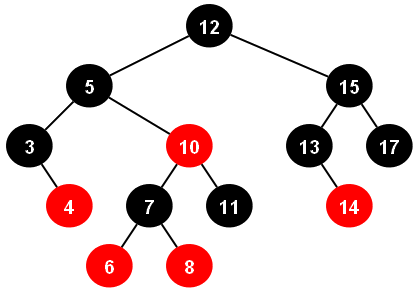
\includegraphics[width=0.45\textwidth]{pictures/redblacktree1.png}
	\caption{RED-BLACK-TREE~\protect\cite{rtoal}}
	\label{fig:rbtree}
\end{figure}

 
Nach \cite[S.311]{tcormen} müssen folgende Regeln für den Rot-Schwarz-Baum eingehalten werden:

\begin{enumerate}
	\item Jeder Knoten ist entweder rot oder schwarz.
	\item Die Wurzel ist schwarz.
	\item Jedes Blatt (NIL) ist schwarz.
	\item Wenn ein Knoten rot ist, dann sind seine beiden Kinder schwarz.
	\item Für jeden Knoten enthalten alle einfachen Pfade, die an diesem Knoten starten und in einem Blatt des Teilbaumes dieses Knotens enden, die gleiche Anzahl schwarzer Knoten. 
\end{enumerate}


Beim Einfügen bzw. Löschen im binäre Baum werden Verbindungen oder Blätter/Knoten verändert. Damit gerät der Baum immer mehr ins Ungleichgewicht. 

Mit den Regeln von RED-BLACK wird mit Hilfe von z.B. Rotationen um das den Parent Knoten, immer für das richtige Gleichgewicht gesorgt.